%=======================+=========================
%================  Online  ================
%=================================================

%------------------------------------------------------------------
\section[Online computing system]{Online computing system \label{sec:online}}

This section describes some of the \GX software and computing systems that are used for both data monitoring and transport to the tape system for permanent storage.

\subsection{Monitoring \label{sec:onlinemonitoring}}

The Online Monitoring system (OMS) consists of several parts that provide for immediate monitoring of the data, as well near term monitoring ($\sim$hours after acquisition). The immediate monitoring is based on the \textit{RootSpy} system\cite{rootspy} written for use in \GX. Figure \ref{fig:online_monitoring_processes} shows a diagram of the processes involved in the RootSpy system and how they couple to the DAQ system using the Event Transfer (ET) software package. ET is part of the CODA DAQ system\cite{coda} and can be used to extract a copy of the data without interfering with the DAQ (i.e. non-blocking mode). The monitoring system utilizes a secondary ET in order to minimize connections to the RAID server running the ER ensuring minimal potential impact to the DAQ through indirect network activity.

\begin{figure}[tbp]
\begin{center}
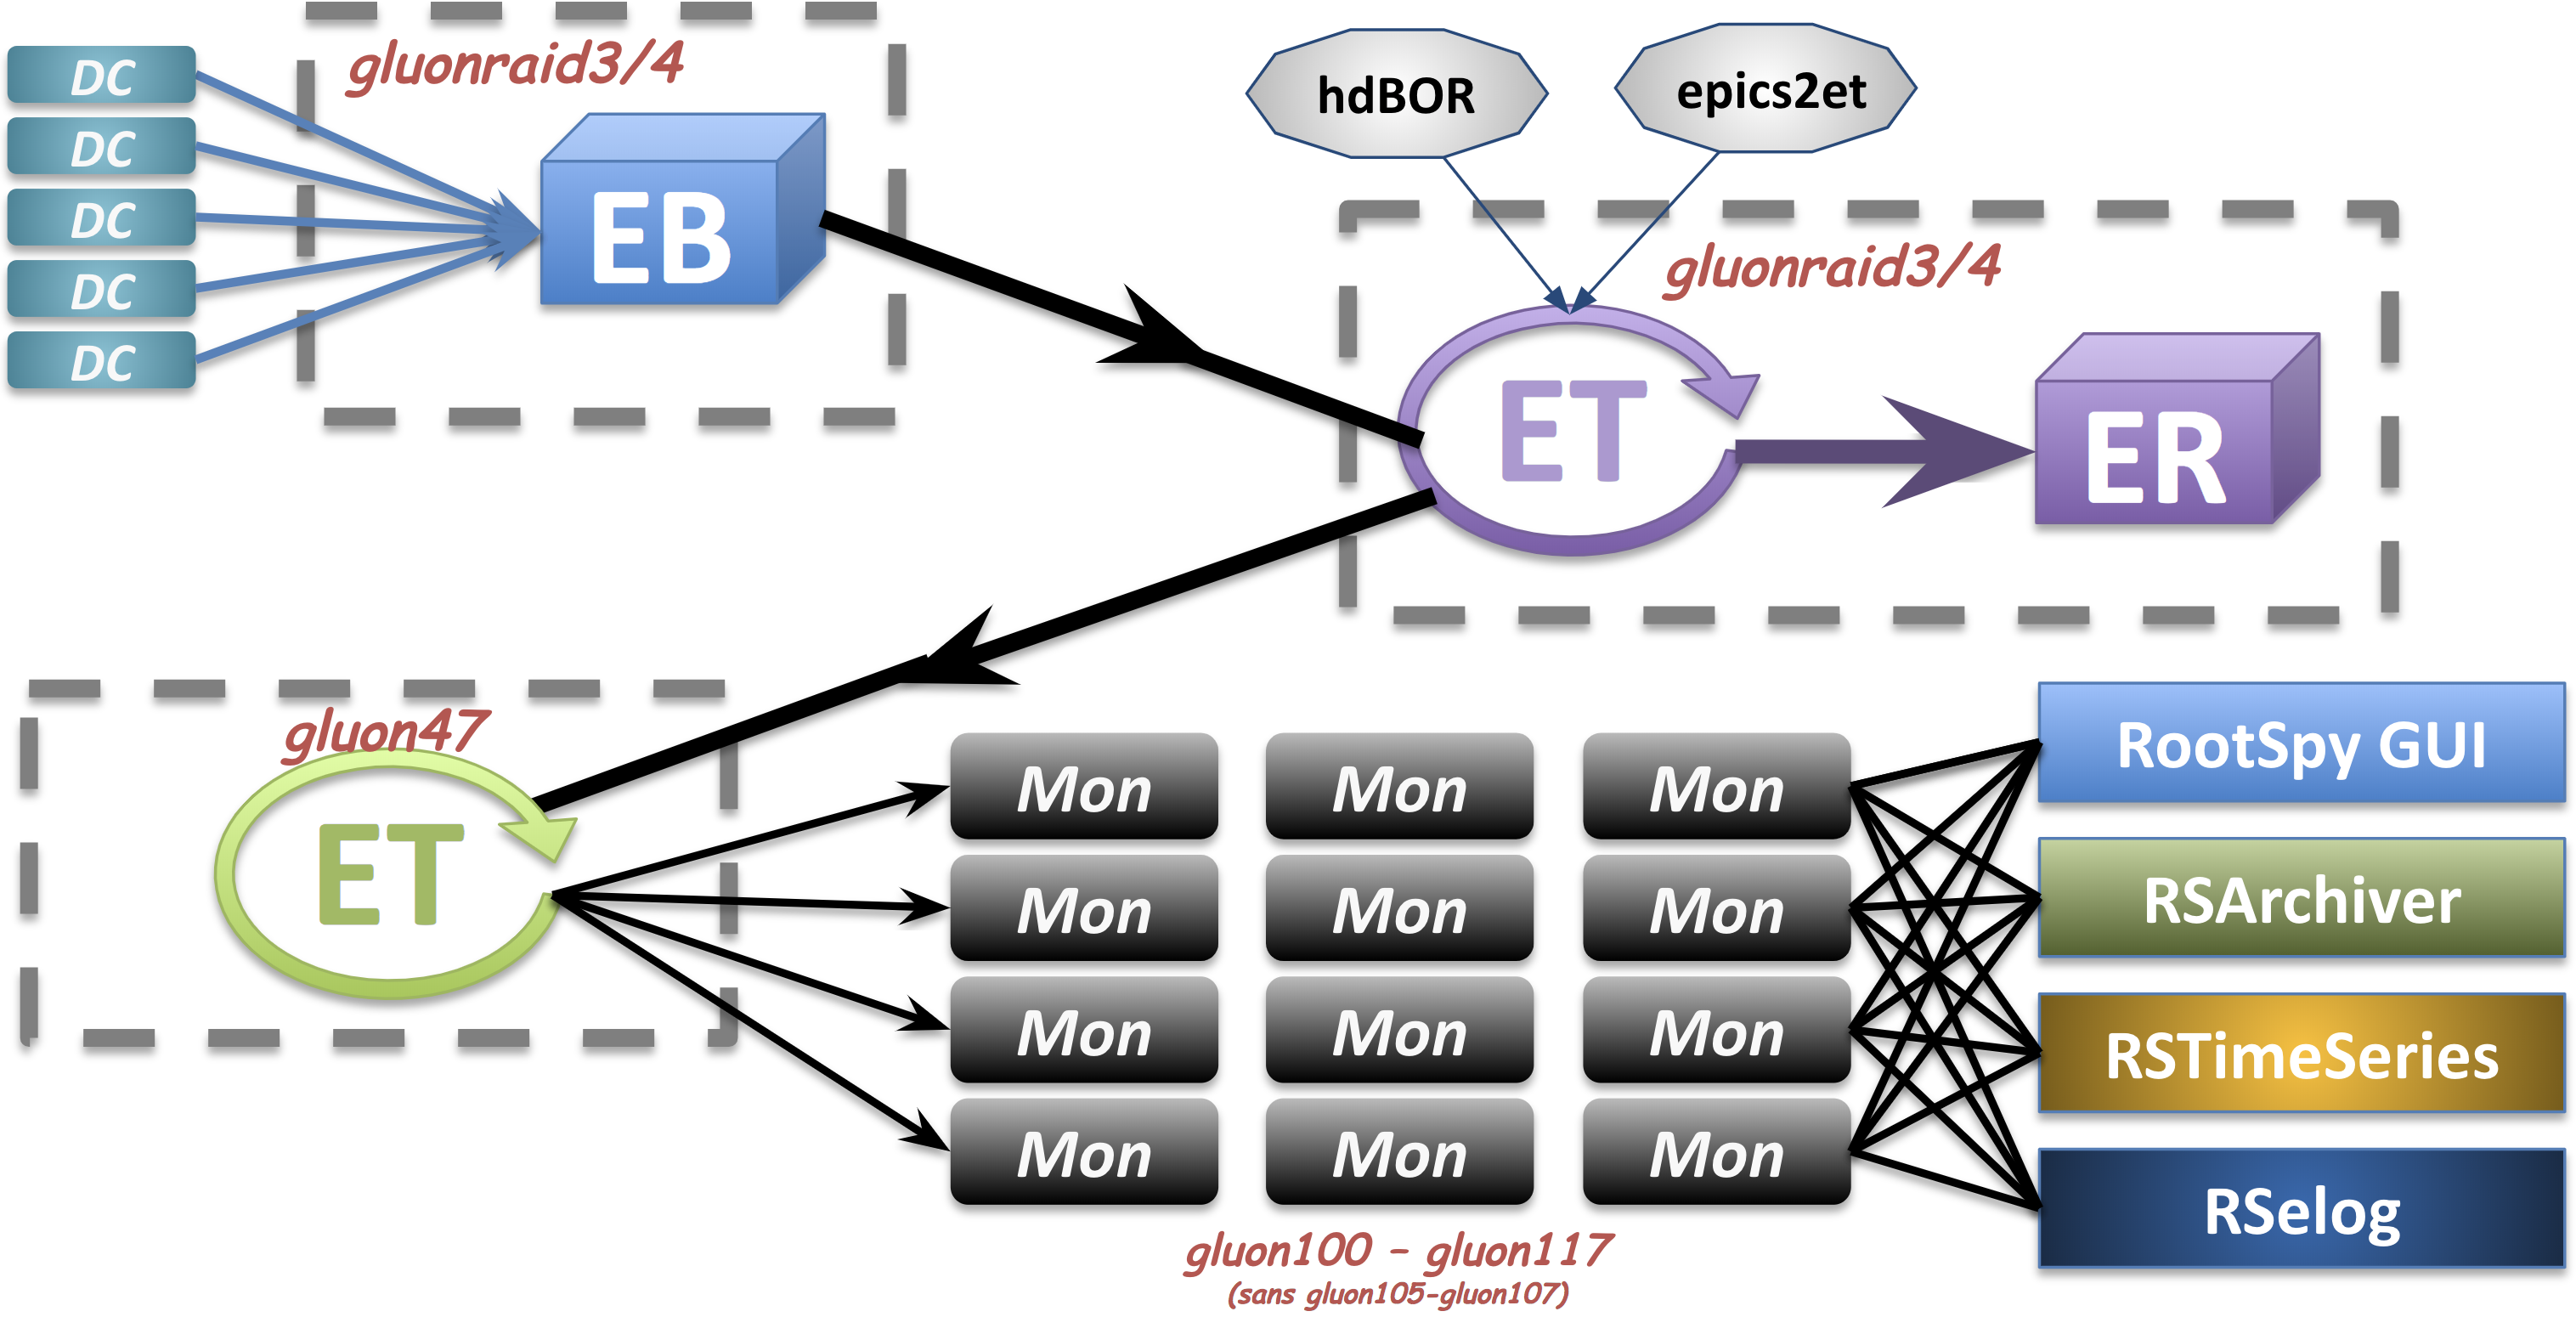
\includegraphics[width=0.99\textwidth]{figures/online_monitoring_processes.png}
\caption{\label{fig:online_monitoring_processes}Diagram of the various processes distributed across several computers in the counting house that make up the online monitoring system. DC, EB, and ER represent the Data Concentrator, Event Builder, and Event Recorder processes respectively in the CODA DAQ system.}   
\end{center}  
\end{figure}

RootSpy was developed at JLab for \GX, though its design is not \GX specific. The system is run on a small farm of computers\footnote{The online monitoring farm consists of eight 2012 era Intel x86\_64 computers with 16 cores+16ht plus six 2016 era Intel x86\_64 computers with 36 cores + 36ht. The monitoring farm uses 40 Gbps (QDR) and 56 Gbps(FDR) IB for the primary interconnect. Note that the DAQ system uses a separate 40 Gbps ethernet network that the farm nodes are not part of.} in the counting house, each processing a small part of the data stream. In total, about 10\% of the data is processed for the low level occupancy plots while roughly 2\% is fully reconstructed for higher level plots. The CODA ET software system is used to distribute the data among the farm computers. Each farm node generates histograms which RootSpy gathers and combines before displaying them to shift workers in a GUI.
%Figure \ref{fig:online_monitoring_rootspy} shows a screen capture of the main RootSpy GUI window along with a window displaying the reference plot for the currently displayed image.
Plots are generally generated via a set of ROOT macros, each responsible for drawing a single page. Most macros divide the page into multiple sections so that multiple plots can be displayed on a single page. The simplest macros display a single occupancy plot. Figure \ref{fig:online_monitoring_PID} shows a page generated by one of the most complex macros. In this page four invariant mass distributions are shown with fits to the distributions that include backgrounds. Values extracted from the fits are printed on the plots for easy quantitative comparison to the reference. 

The main RootSpy window allows pages to be grouped into tabs and for users to step through the pages either via mouse click or automatically every few seconds. Reference pages are displayed in a separate window next to the main GUI allowing shift workers to visually compare for discrepancies. Shift workers may use the GUI to set the currently displayed page as the new reference for that particular page. An e-mail is automatically sent when this is done to a list of addresses associated with the page. (Actually from special comment lines embedded in the macro itself). The e-mail includes the old and new reference images so that system experts receiving the e-mail can see when a new reference is installed and how it differs from the previous.

Macros are passed into the GUI using the same xMsg\cite{xmsg} publish subscribe messaging system used to transport histogram objects. The macros are compiled into plugins as C++ strings by the build system. The build system recognizes ROOT macro files in the plugin source directory (via the .C suffix) and automatically generates C++ code that contains the macro and code to register it with the RootSpy system. This is done to ensure that a macro is always in sync with the histograms it displays since the former is linked in the same binary as the routines that produce the latter.

\begin{figure}[tbp]
\begin{center}
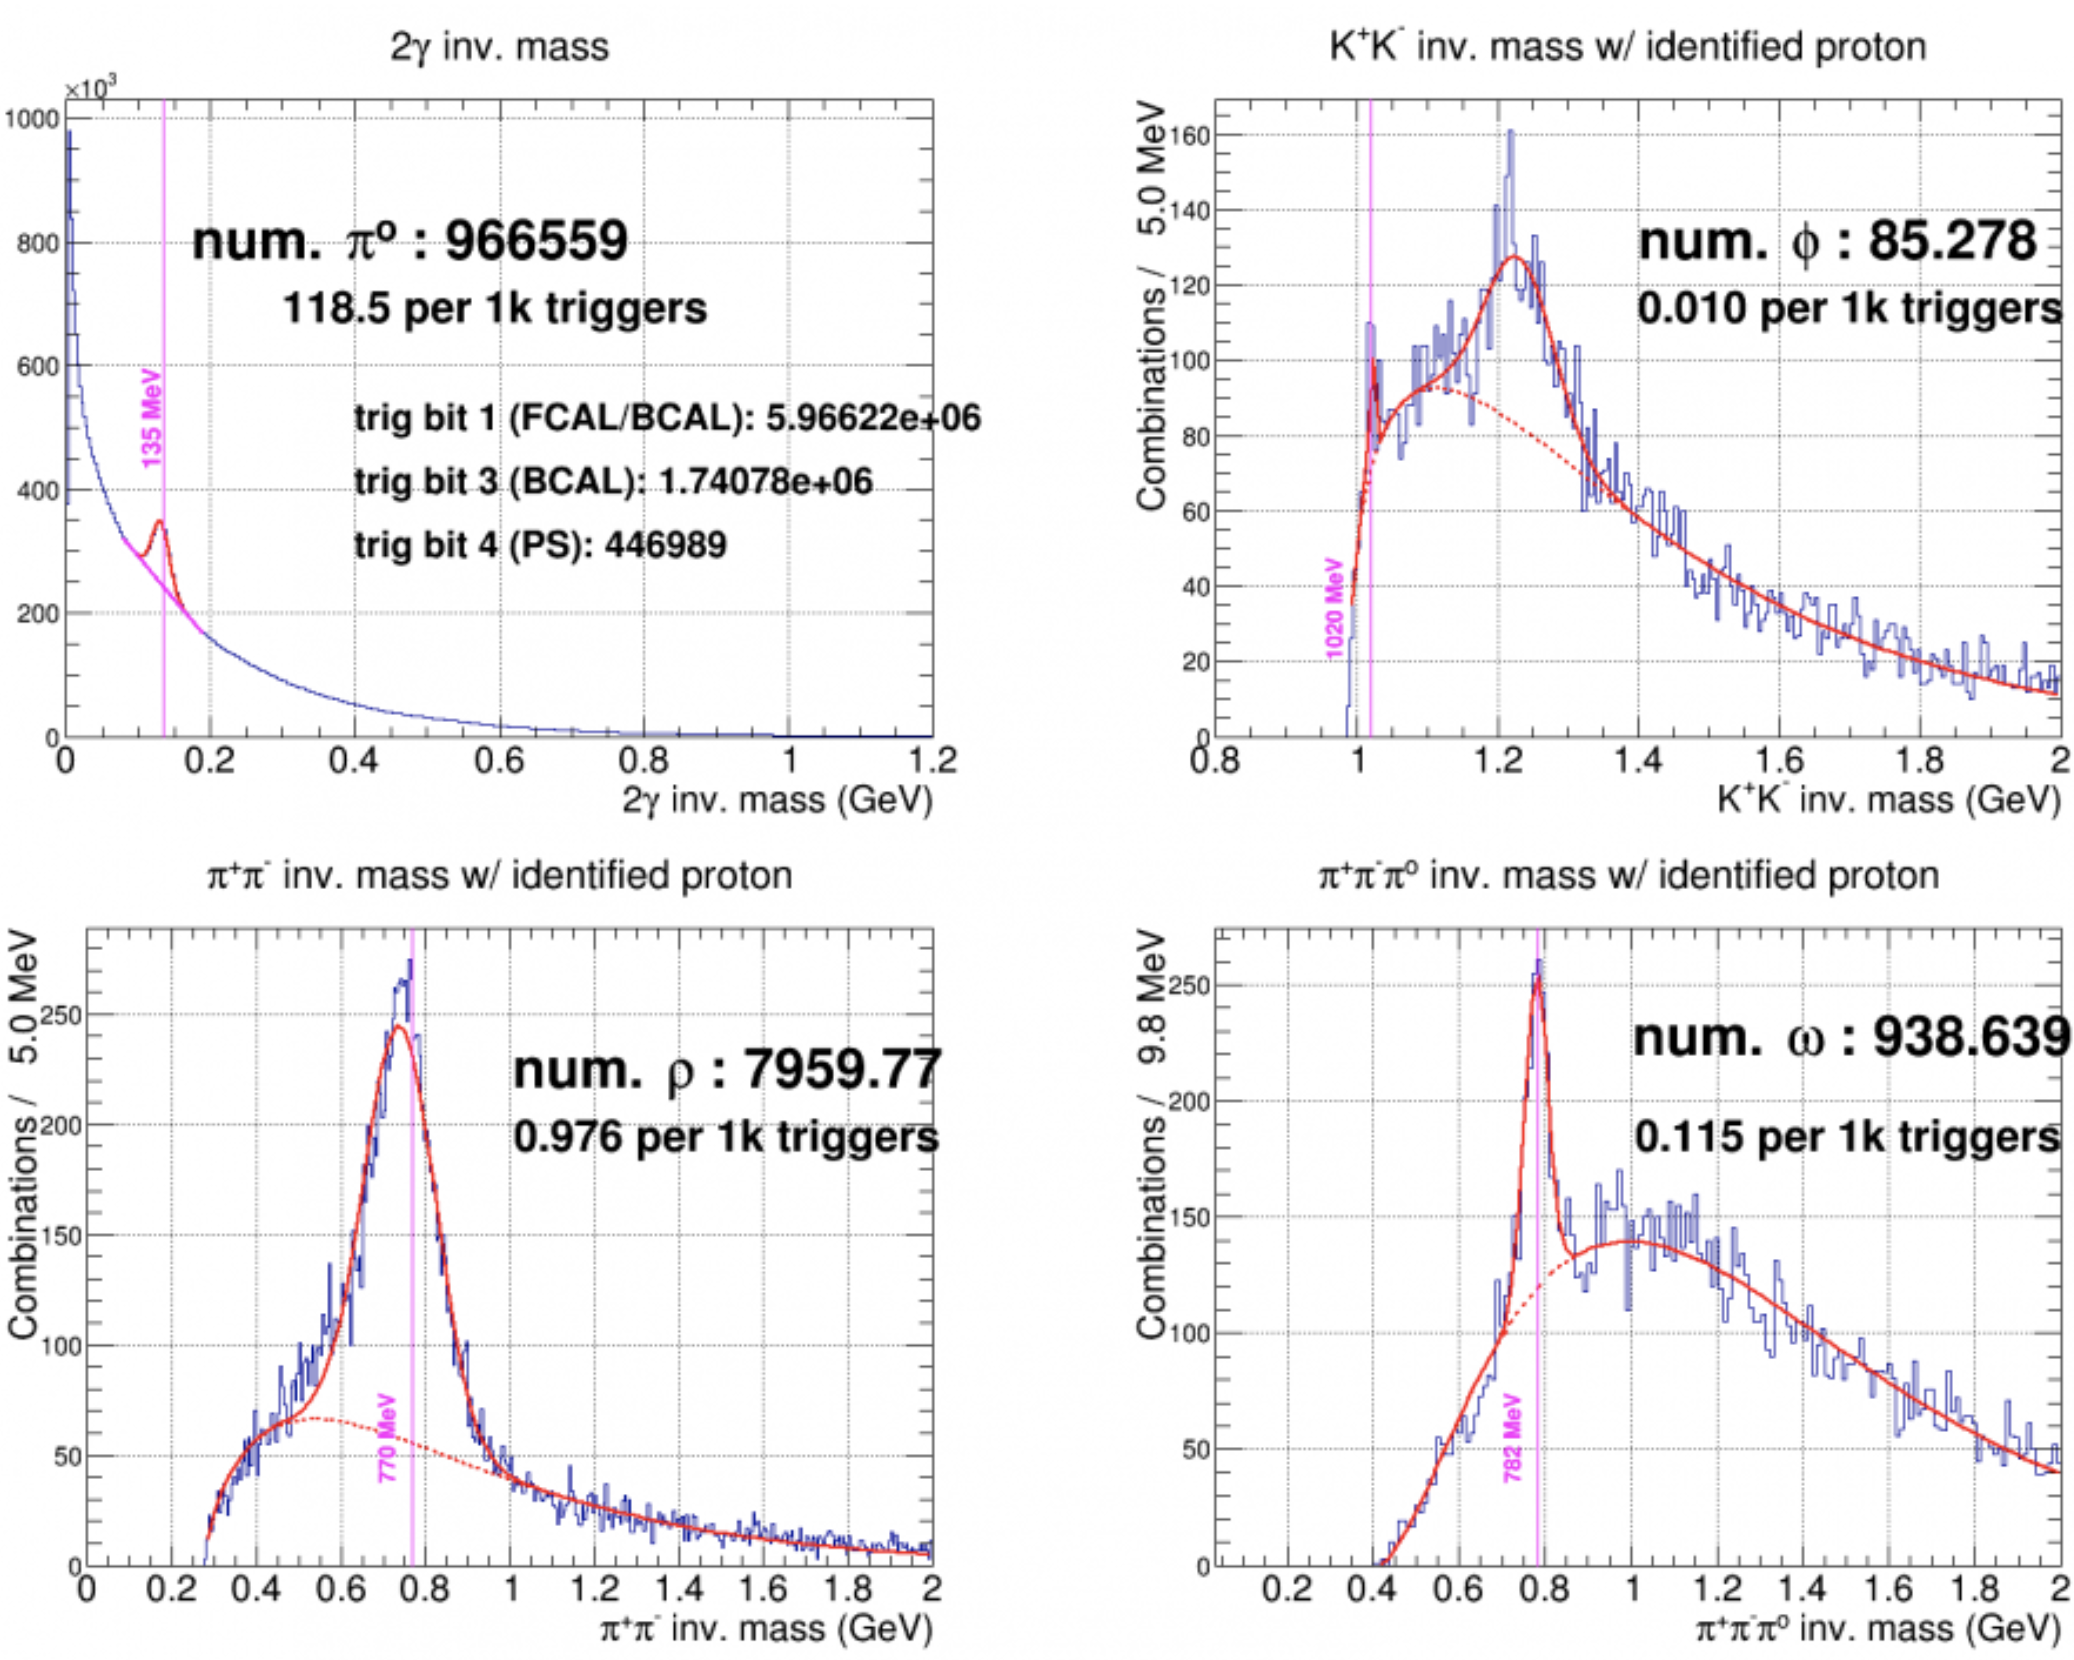
\includegraphics[width=0.99\textwidth]{figures/online_monitoring_PID.png}
\caption{\label{fig:online_monitoring_PID}Invariant mass distributions showing $\pi^\circ$, $\omega$, $\rho$, and $\phi$ particles. These plots were generated online in about 1hr 40min by looking at roughly 2\% of the data stream.}   
\end{center}  
\end{figure}

% \begin{figure}[tbp]
% \begin{center}
% 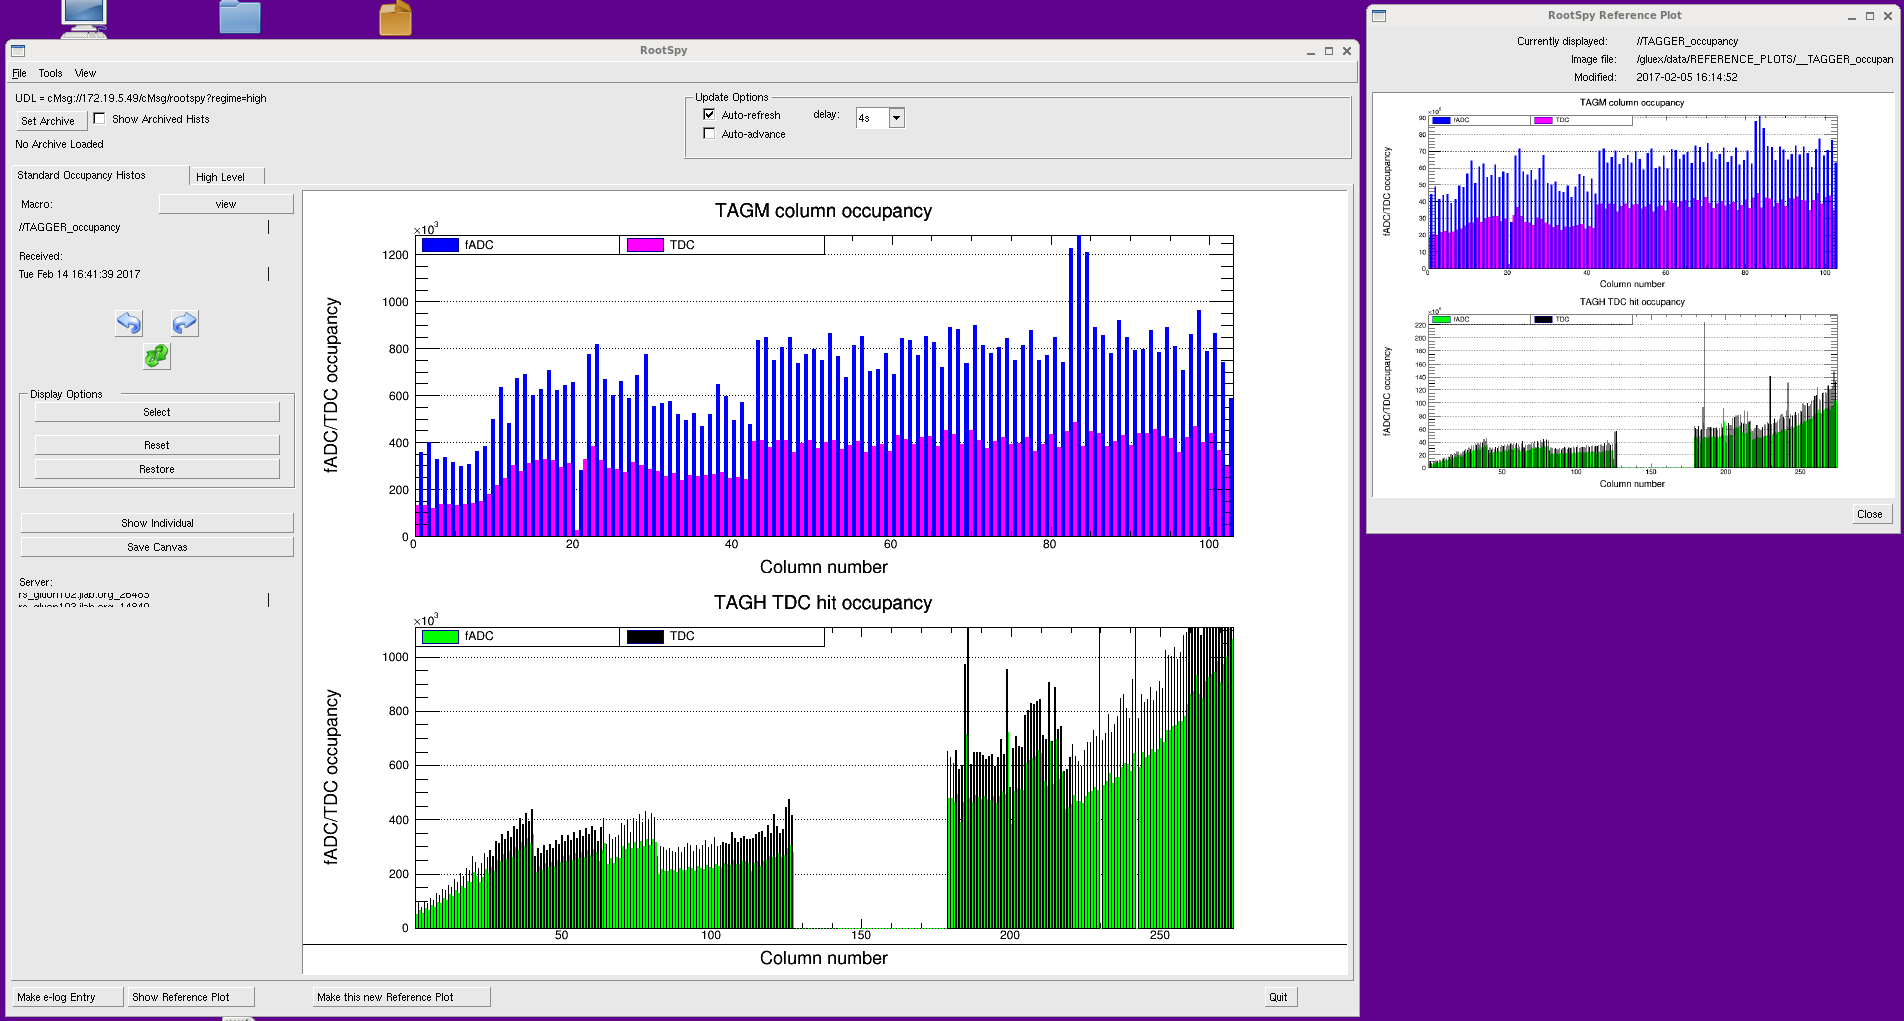
\includegraphics[width=0.99\textwidth]{figures/online_monitoring_rootspy.png}
% \label{fig:online_monitoring_rootspy}
% \caption{Screen capture of the RootSpy GUI program main window and the reference image in the upper right.}   
% \end{center}  
% \end{figure}

Each farm node runs a JANA\cite{jana_v0_8_1b} process that links the same \GX libraries used in the final reconstruction of \GX data. Three of the monitoring computers are dedicated to ``occupancy'' plots which allows them to process events at a much higher rate since they do not perform full event reconstruction. The remaining eleven monitoring computers produce these same plots and in addition do perform full event reconstruction. The system was able to perform full reconstruction immediately online on about 2\%-3\% of the data stream while hit level only occupancy plots were produced for 10\%-15\% during phase I \GX running.


% \begin{figure}[tbp]
% \begin{center}
% 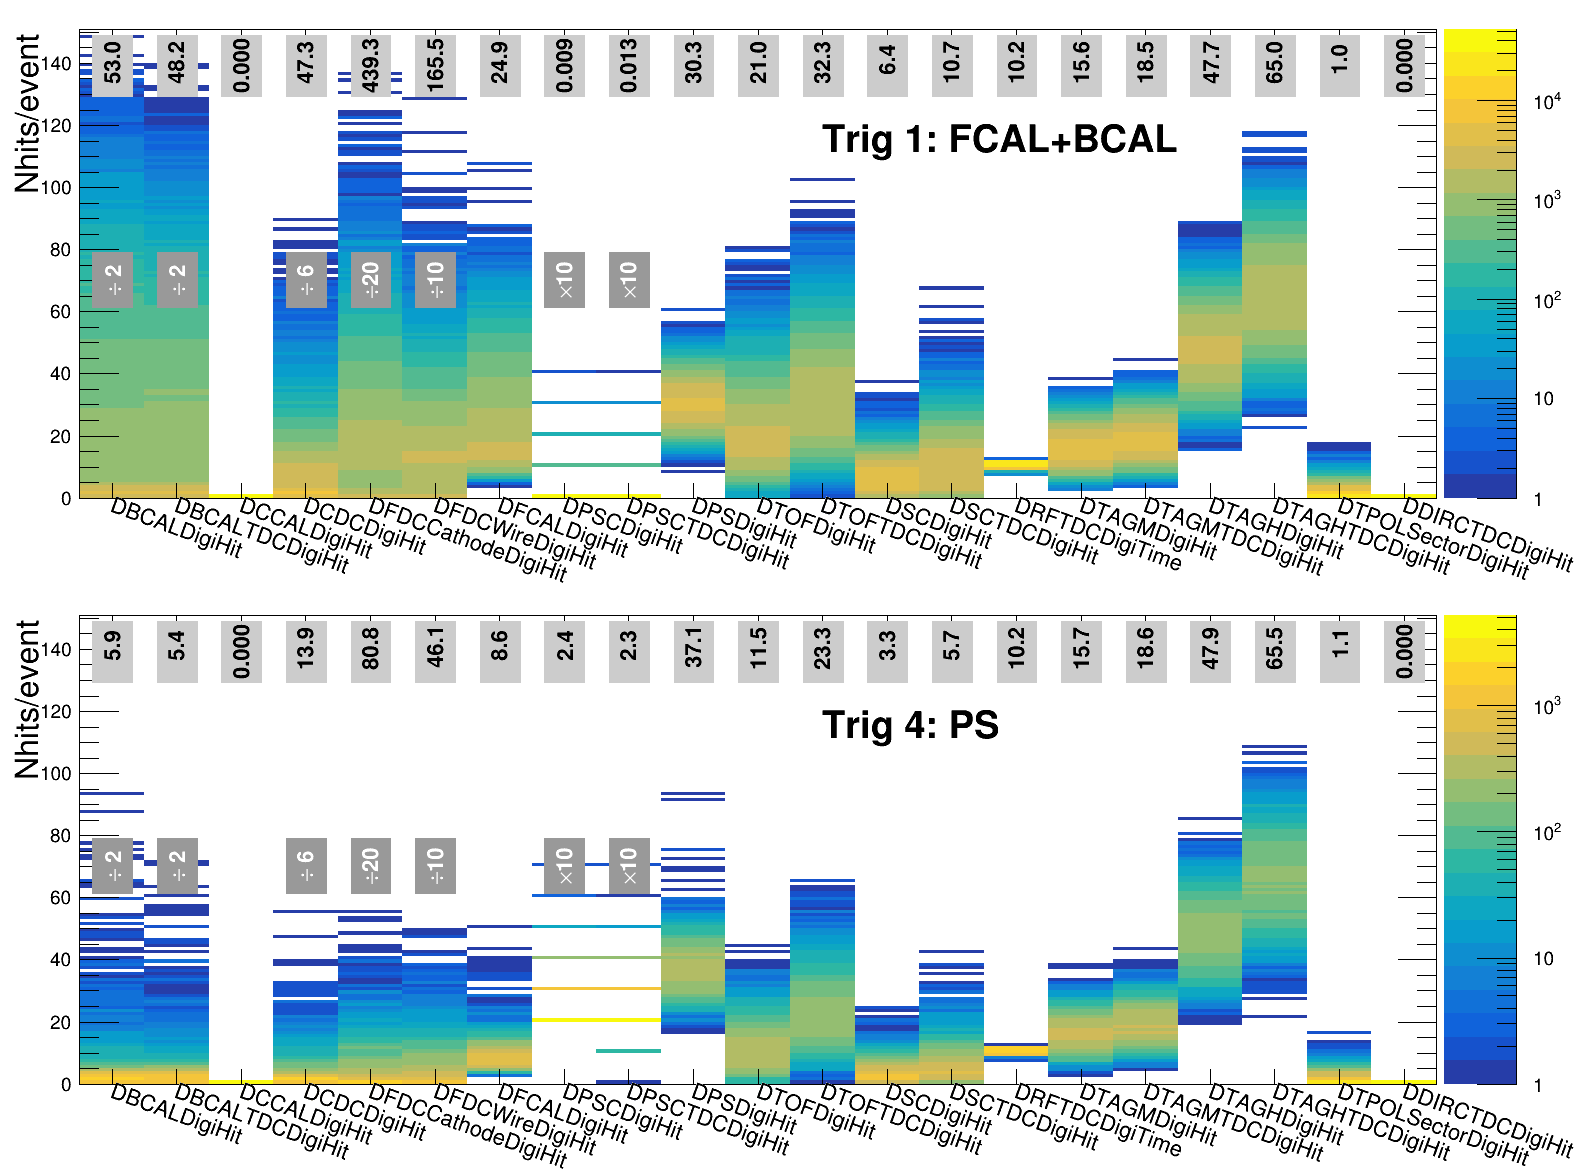
\includegraphics[width=0.99\textwidth]{figures/online_monitoring_digihits.png}
% \label{fig:online_monitoring_digihits}
% \caption{Example monitoring plot showing the number of low-level hit objects per event separated by trigger type. Some have the y-values are scaled by factors shown in the grey boxes so that they comfortably fit on the same plot.}   
% \end{center}  
% \end{figure}

In addition to the RootSpy GUI, several other client programs exist that consume the histograms being produced by the farm nodes. One of these is the RSTimeSeries program. This program runs in the background periodically running a subset of macros that contain special calls to insert data into an InfluxDB time series database. This provides a web-accessible strip chart of detector hit rates and reconstructed quantities like number of $\rho$s per 1k triggers. The RSArchiver program gathers summed histograms and periodically writes them to a ROOT file for permanent archival. The archive file is used to generate a set of image files using the same ROOT macros used by the RootSpy GUI. These are displayed in the Plot Browser\footnote{https://halldweb.jlab.org/data\_monitoring/Plot\_Browser.html} website for easy comparison of plots for different runs as well as with the same plots produced during offline analysis. The first five files (100GB) of each run are automatically pinned to disk in the JLab Computing Center after being transported there for permanent tape storage. Jobs are automatically submitted for these files to the JLab SciComp farm to perform full reconstruction on these files and produce a set of image files that are also displayed in Plot Browser under the title ``Incoming Data''.

%Examples of these are shown in figures \ref{fig:online_monitoring_grafana1} and \ref{fig:online_monitoring_grafana2}. Figure \ref{fig:online_monitoring_grafana2} shows a strip chart of the particles per 1k triggers extracted from the same macro used to draw figure \ref{fig:online_monitoring_PID}.

% \begin{figure}[tbp]
% \begin{center}
% 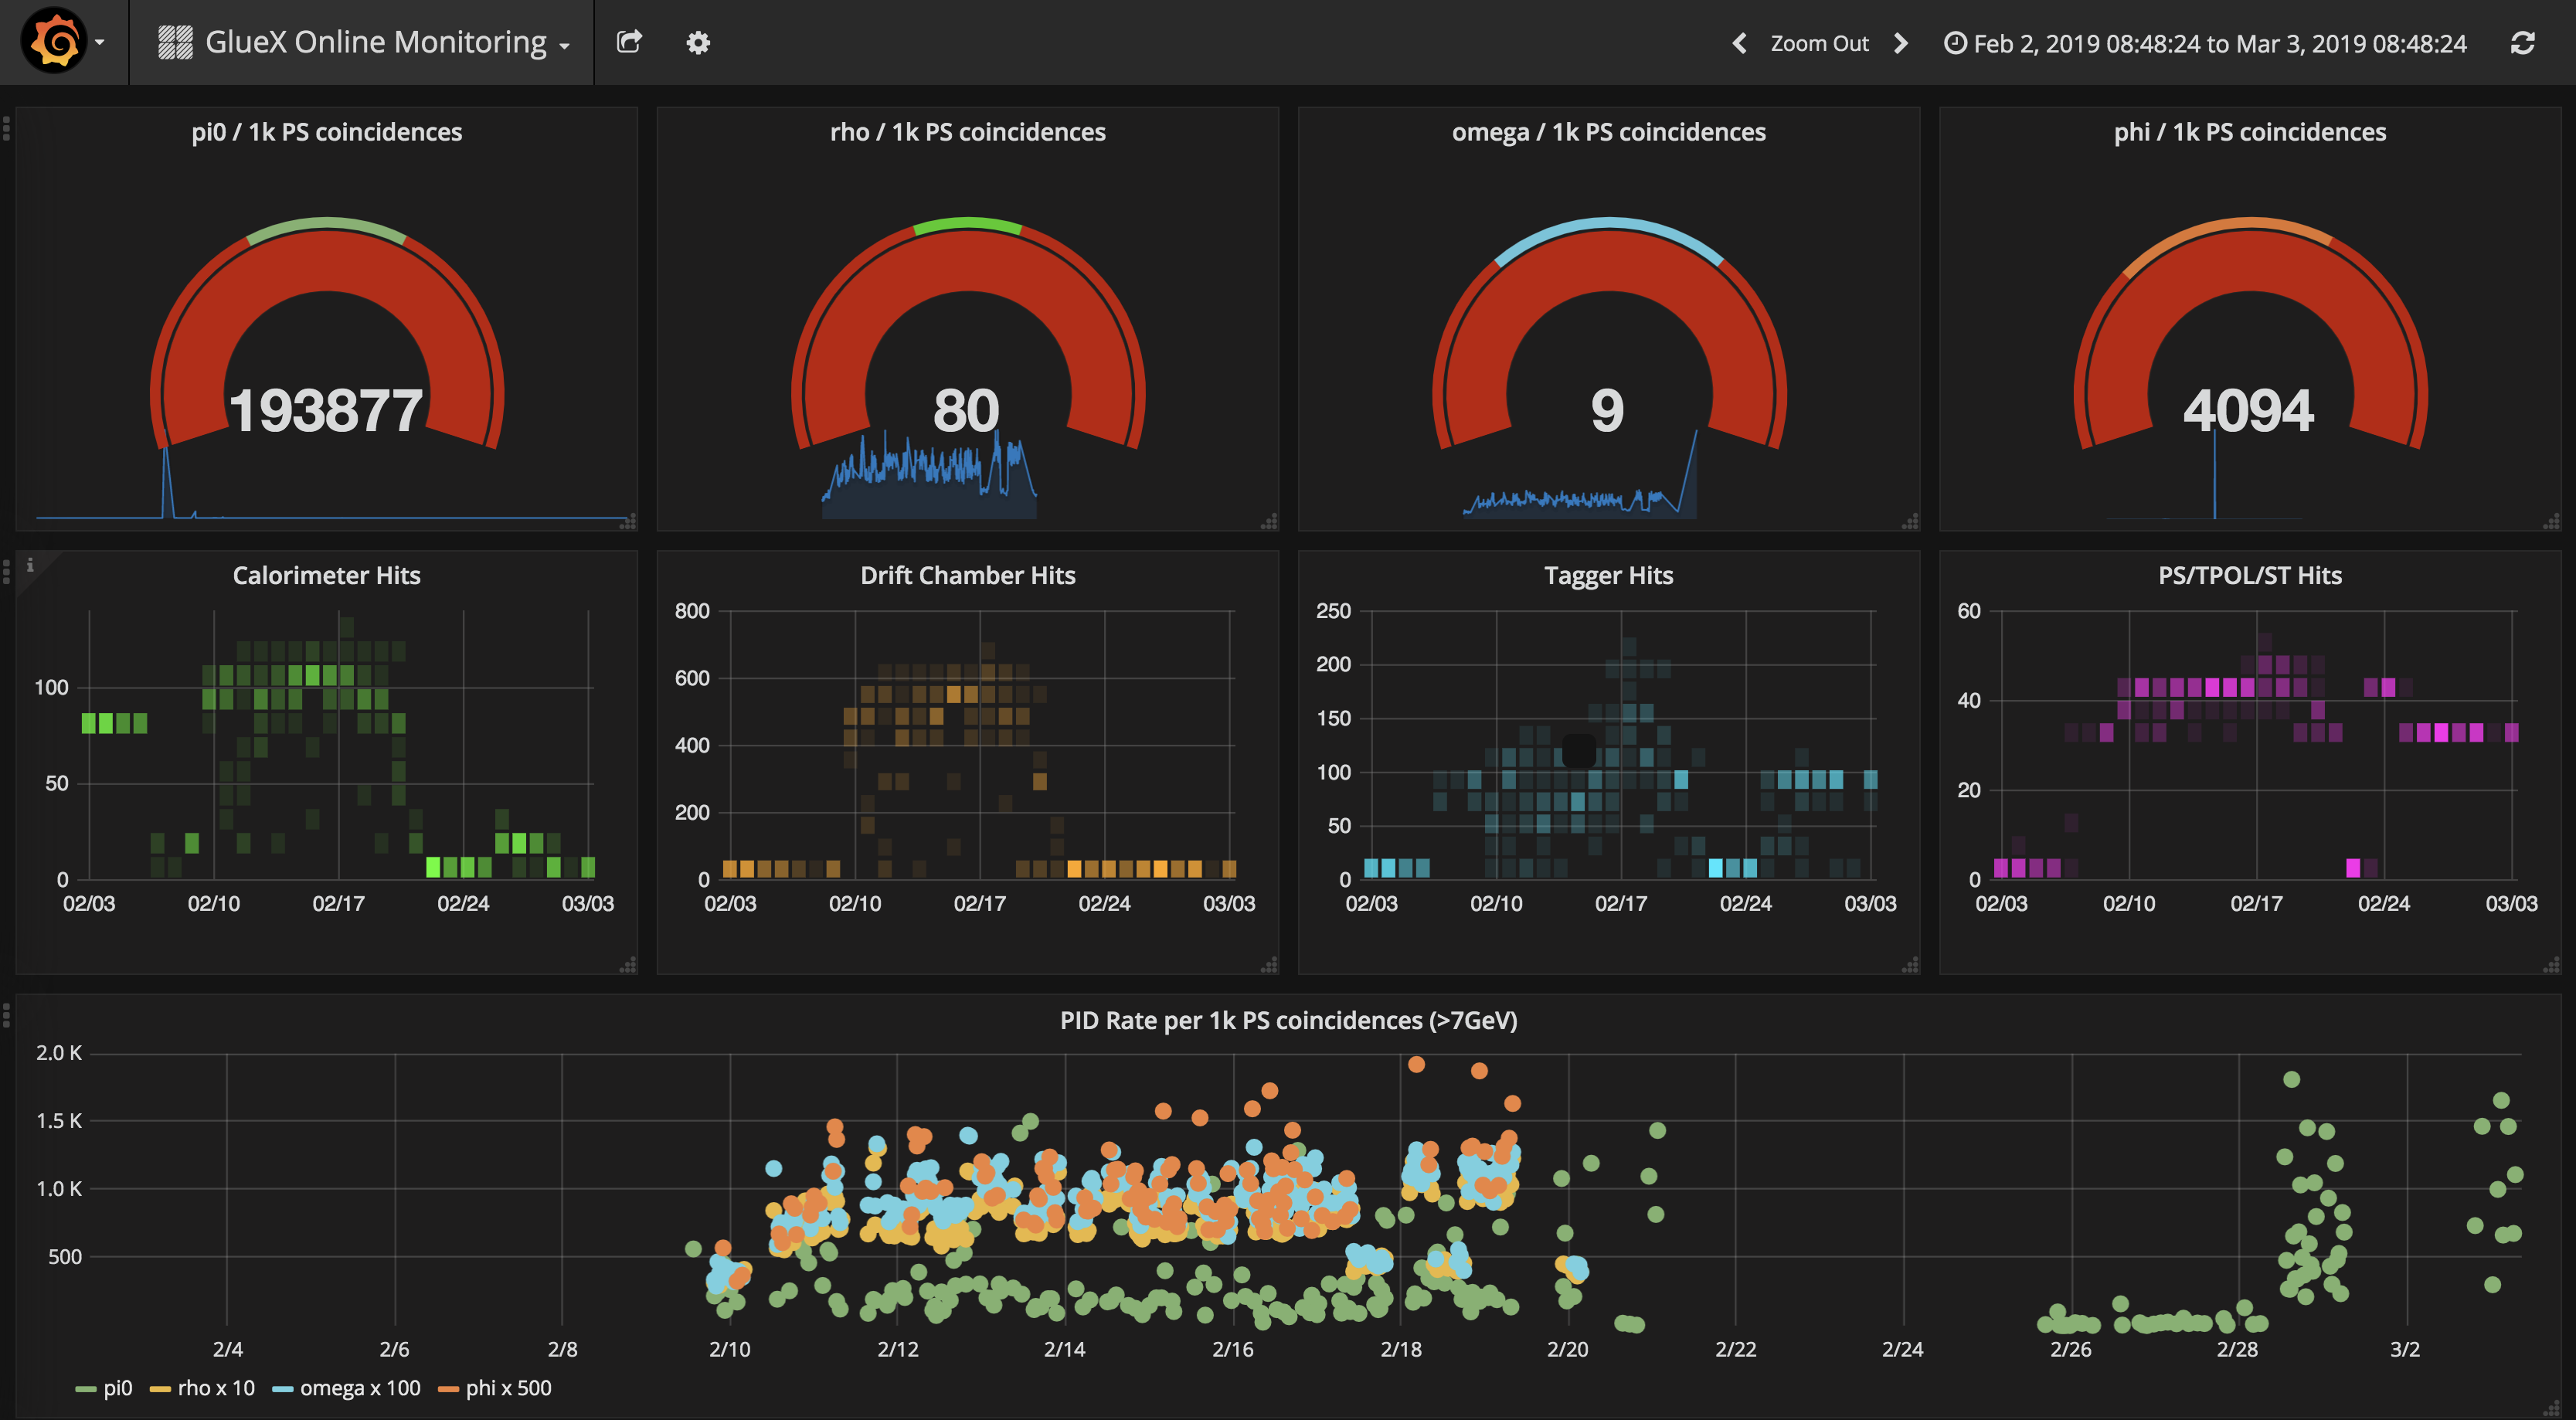
\includegraphics[width=0.99\textwidth]{figures/online_monitoring_grafana1.png}
% \label{fig:online_monitoring_grafana1}
% \caption{Screen capture of Grafana driven web site showing reconstructed particle rates and detector hit rates as a function of time.}
% \end{center}  
% \end{figure}

% \begin{figure}[tbp]
% \begin{center}
% 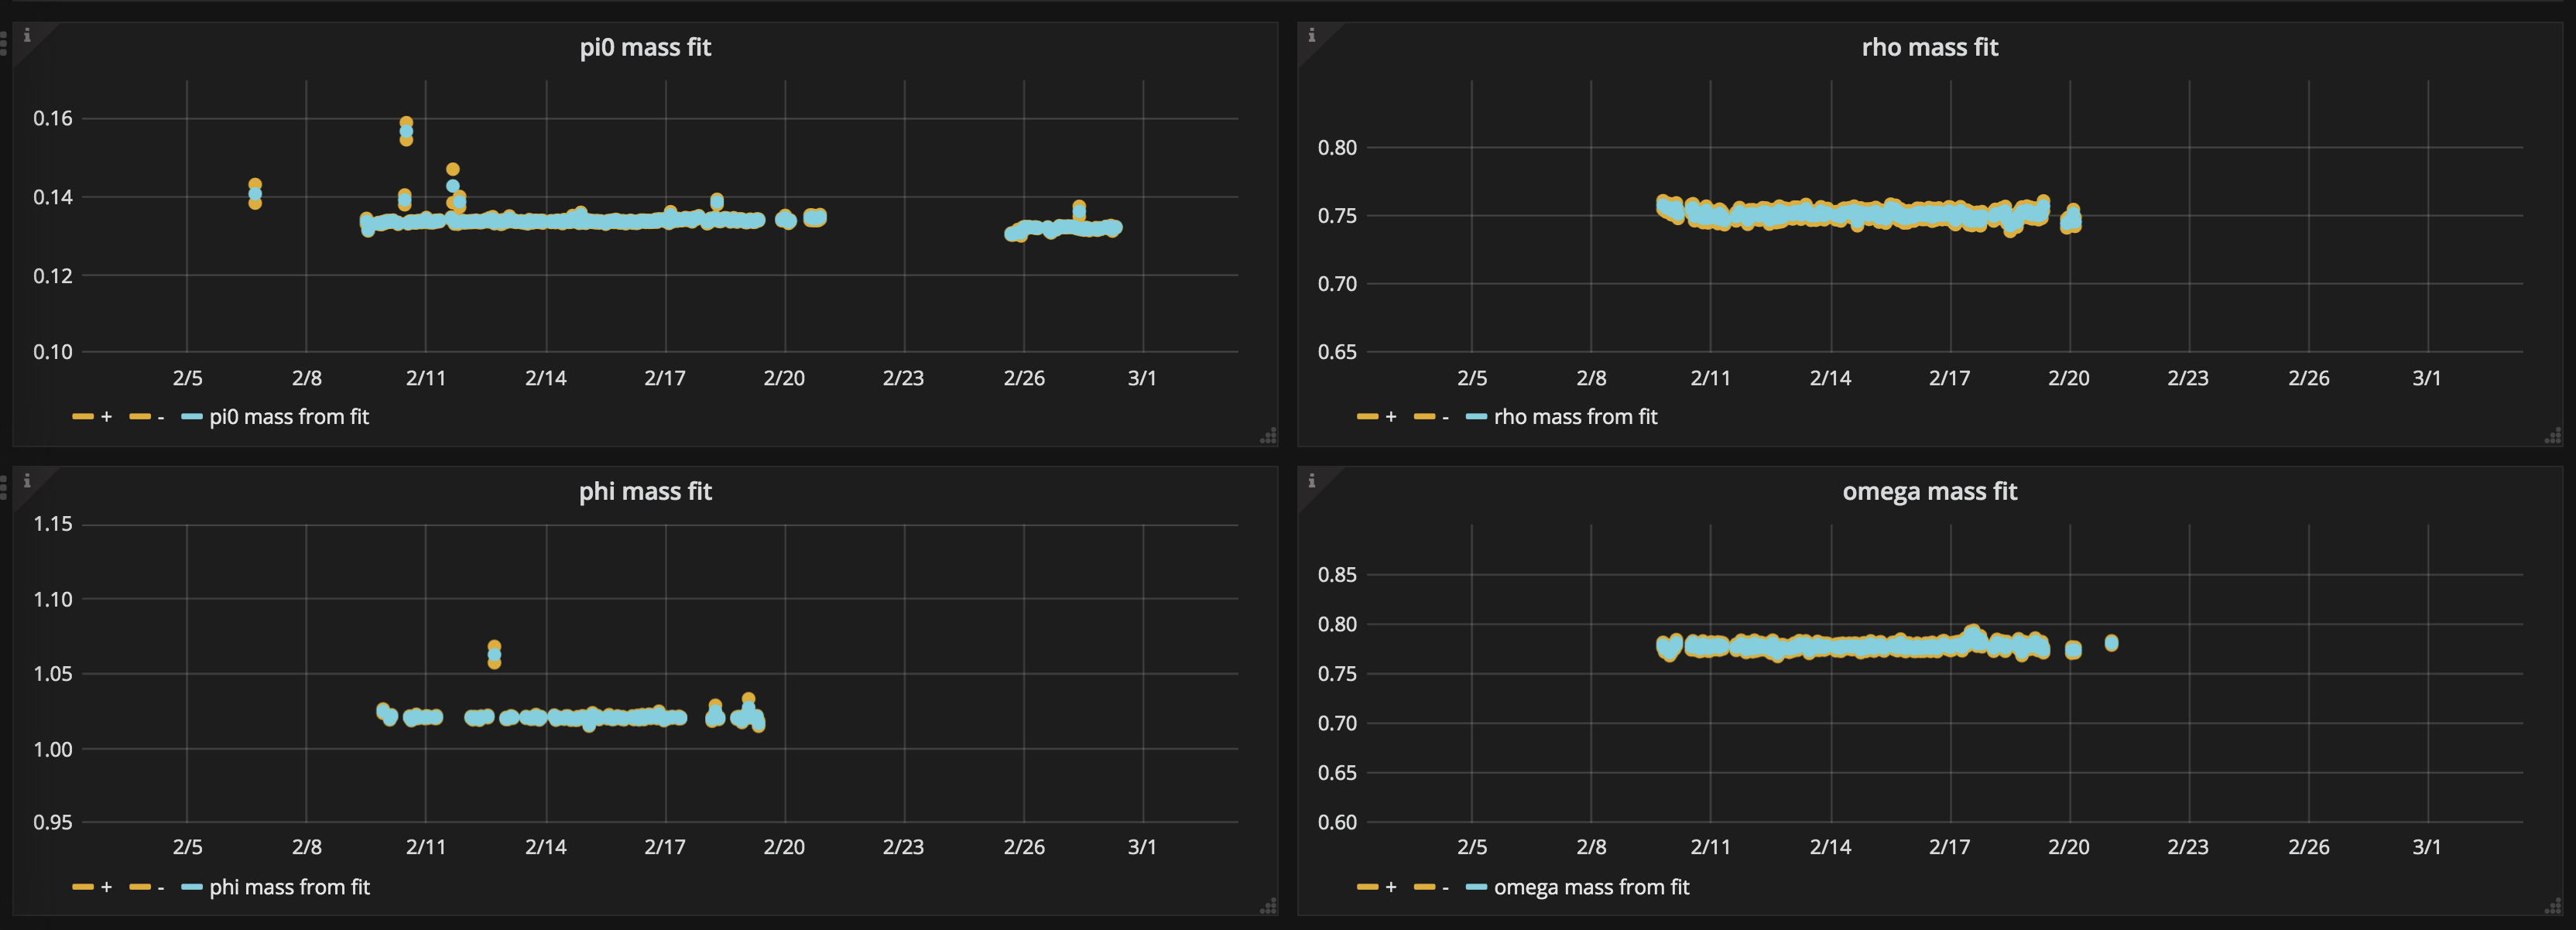
\includegraphics[width=0.99\textwidth]{figures/online_monitoring_grafana2.png}
% \label{fig:online_monitoring_grafana2}
% \caption{Online strip charts of particle rates per trigger. The online monitoring system does full reconstruction of 2\%-3\% of events as the data is acquired.}   
% \end{center}  
% \end{figure}

% \begin{figure}[tbp]
% \begin{center}
% 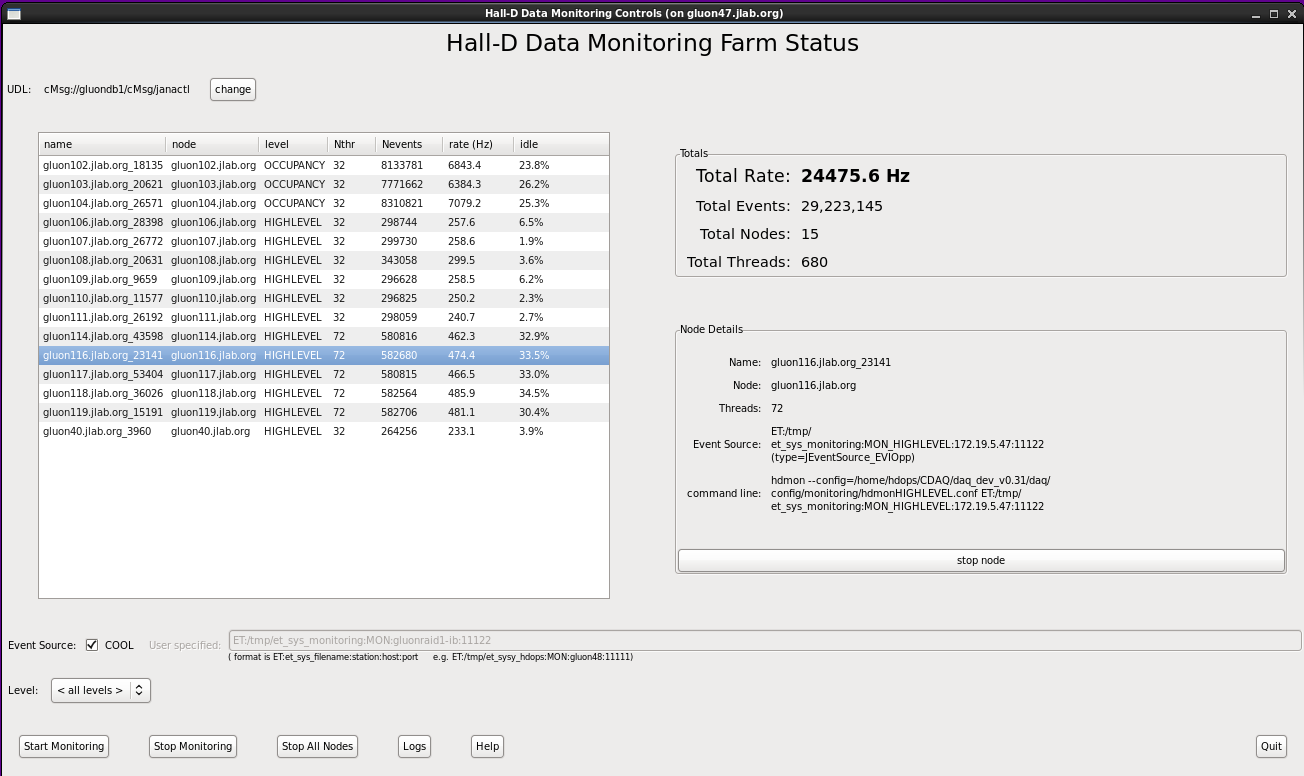
\includegraphics[width=0.99\textwidth]{figures/online_monitoring_hdmongui.png}
% \label{fig:online_monitoring_hdmongui}
% \caption{GUI interface to online monitoring system.}   
% \end{center}  
% \end{figure}


%------------------------------------------------------------------
\subsection{Data Transport and Storage \label{sec:onlineprocessing}}

\GX Phase I generated production data at rates up to 650MB/s. The data was temporarily stored on large RAID-6 disk arrays and then copied to an LT0 tape system for long term storage. One of two RAID servers was used for each run period with sizes of 264TB and 310TB. Which server was used was alternated between run periods. Each of the servers was broken into four partitions with each partition made up of a dedicated set of physical disks. The partition being written to was rotated between runs through the use of symlinks. This helped to minimize head thrashing on disks by only reading from the partitions not currently being written to. Figure \ref{fig:online_dataflow} shows an overview of the raw data flow occurring between the DAQ and tape systems. A cron job would scan the \textit{active} directory for completed data files and move any it found into the \textit{volatile} directory (on the same partition). A hard link would then be made in the \textit{staging directory}. Software provided by the JLab IT division would transport any files found in \textit{staging} to tape and then delete them upon successful transfer. Files in \textit{volatile} would be deleted via another cron job as needed to free up space. This system allowed all RAID partitions to be kept at roughly 80\% full at all times with the most recent data. This was useful for performing calibrations or small analysis jobs in the counting house during beam off times. An additional copy of the first 3 files of each run was made to a smaller RAID disk so that an easily accessible sample of each run could be maintained in the counting house.

The auto-deletion system of the files in the \textit{volatile} directory was based on choosing files with the largest size $\times$ access time. This meant recently accessed files would be kept longer, most likely because they were in use for calibrations or special studies. A typical raw data file would exist on the RAID system during production data taking for 3-5 days, though it would be copied to the tape system within several hours of having been created.

The data volumes stored to tape are shown in table \ref{tab:online_data_volumes} in units of petabytes(PB). Lines marked ``actual'' are values taken from the tape storage system. Lines marked ``model'' come from the \GX computing model\cite{gx3821}.

\begin{table}[]
    \centering
    \begin{tabular}{|l|c|c|c|c|c|}
    \hline
                           & \textbf{2016}  & \textbf{2017}  & \textbf{2018} \\
    \hline
    actual (raw data only) & 0.624 & 0.914 & 3.107 \\
    \hline
     model (raw data only) &       & 0.863 & 3.172 \\
    \hline
    \hline
    actual (production)    & 0.55  & 1.256 & 1.206 \\
    \hline
     model (production)    &       & 0.607 & 3.084 \\
    \hline
    \end{tabular}
    \caption{\GX Data volumes by year. All values are in petabytes(PB). Most years include two run periods. The lines marked \textit{model} are calculated from the \GX Computing Model\cite{gx3821}. ``raw data only'' represents data generated by the DAQ system (not including the backup copy). ``production'' represents all data derived from that (reconstructed values and ROOT trees). }
    \label{tab:online_data_volumes}
\end{table}


\begin{figure}[tbp]
\begin{center}
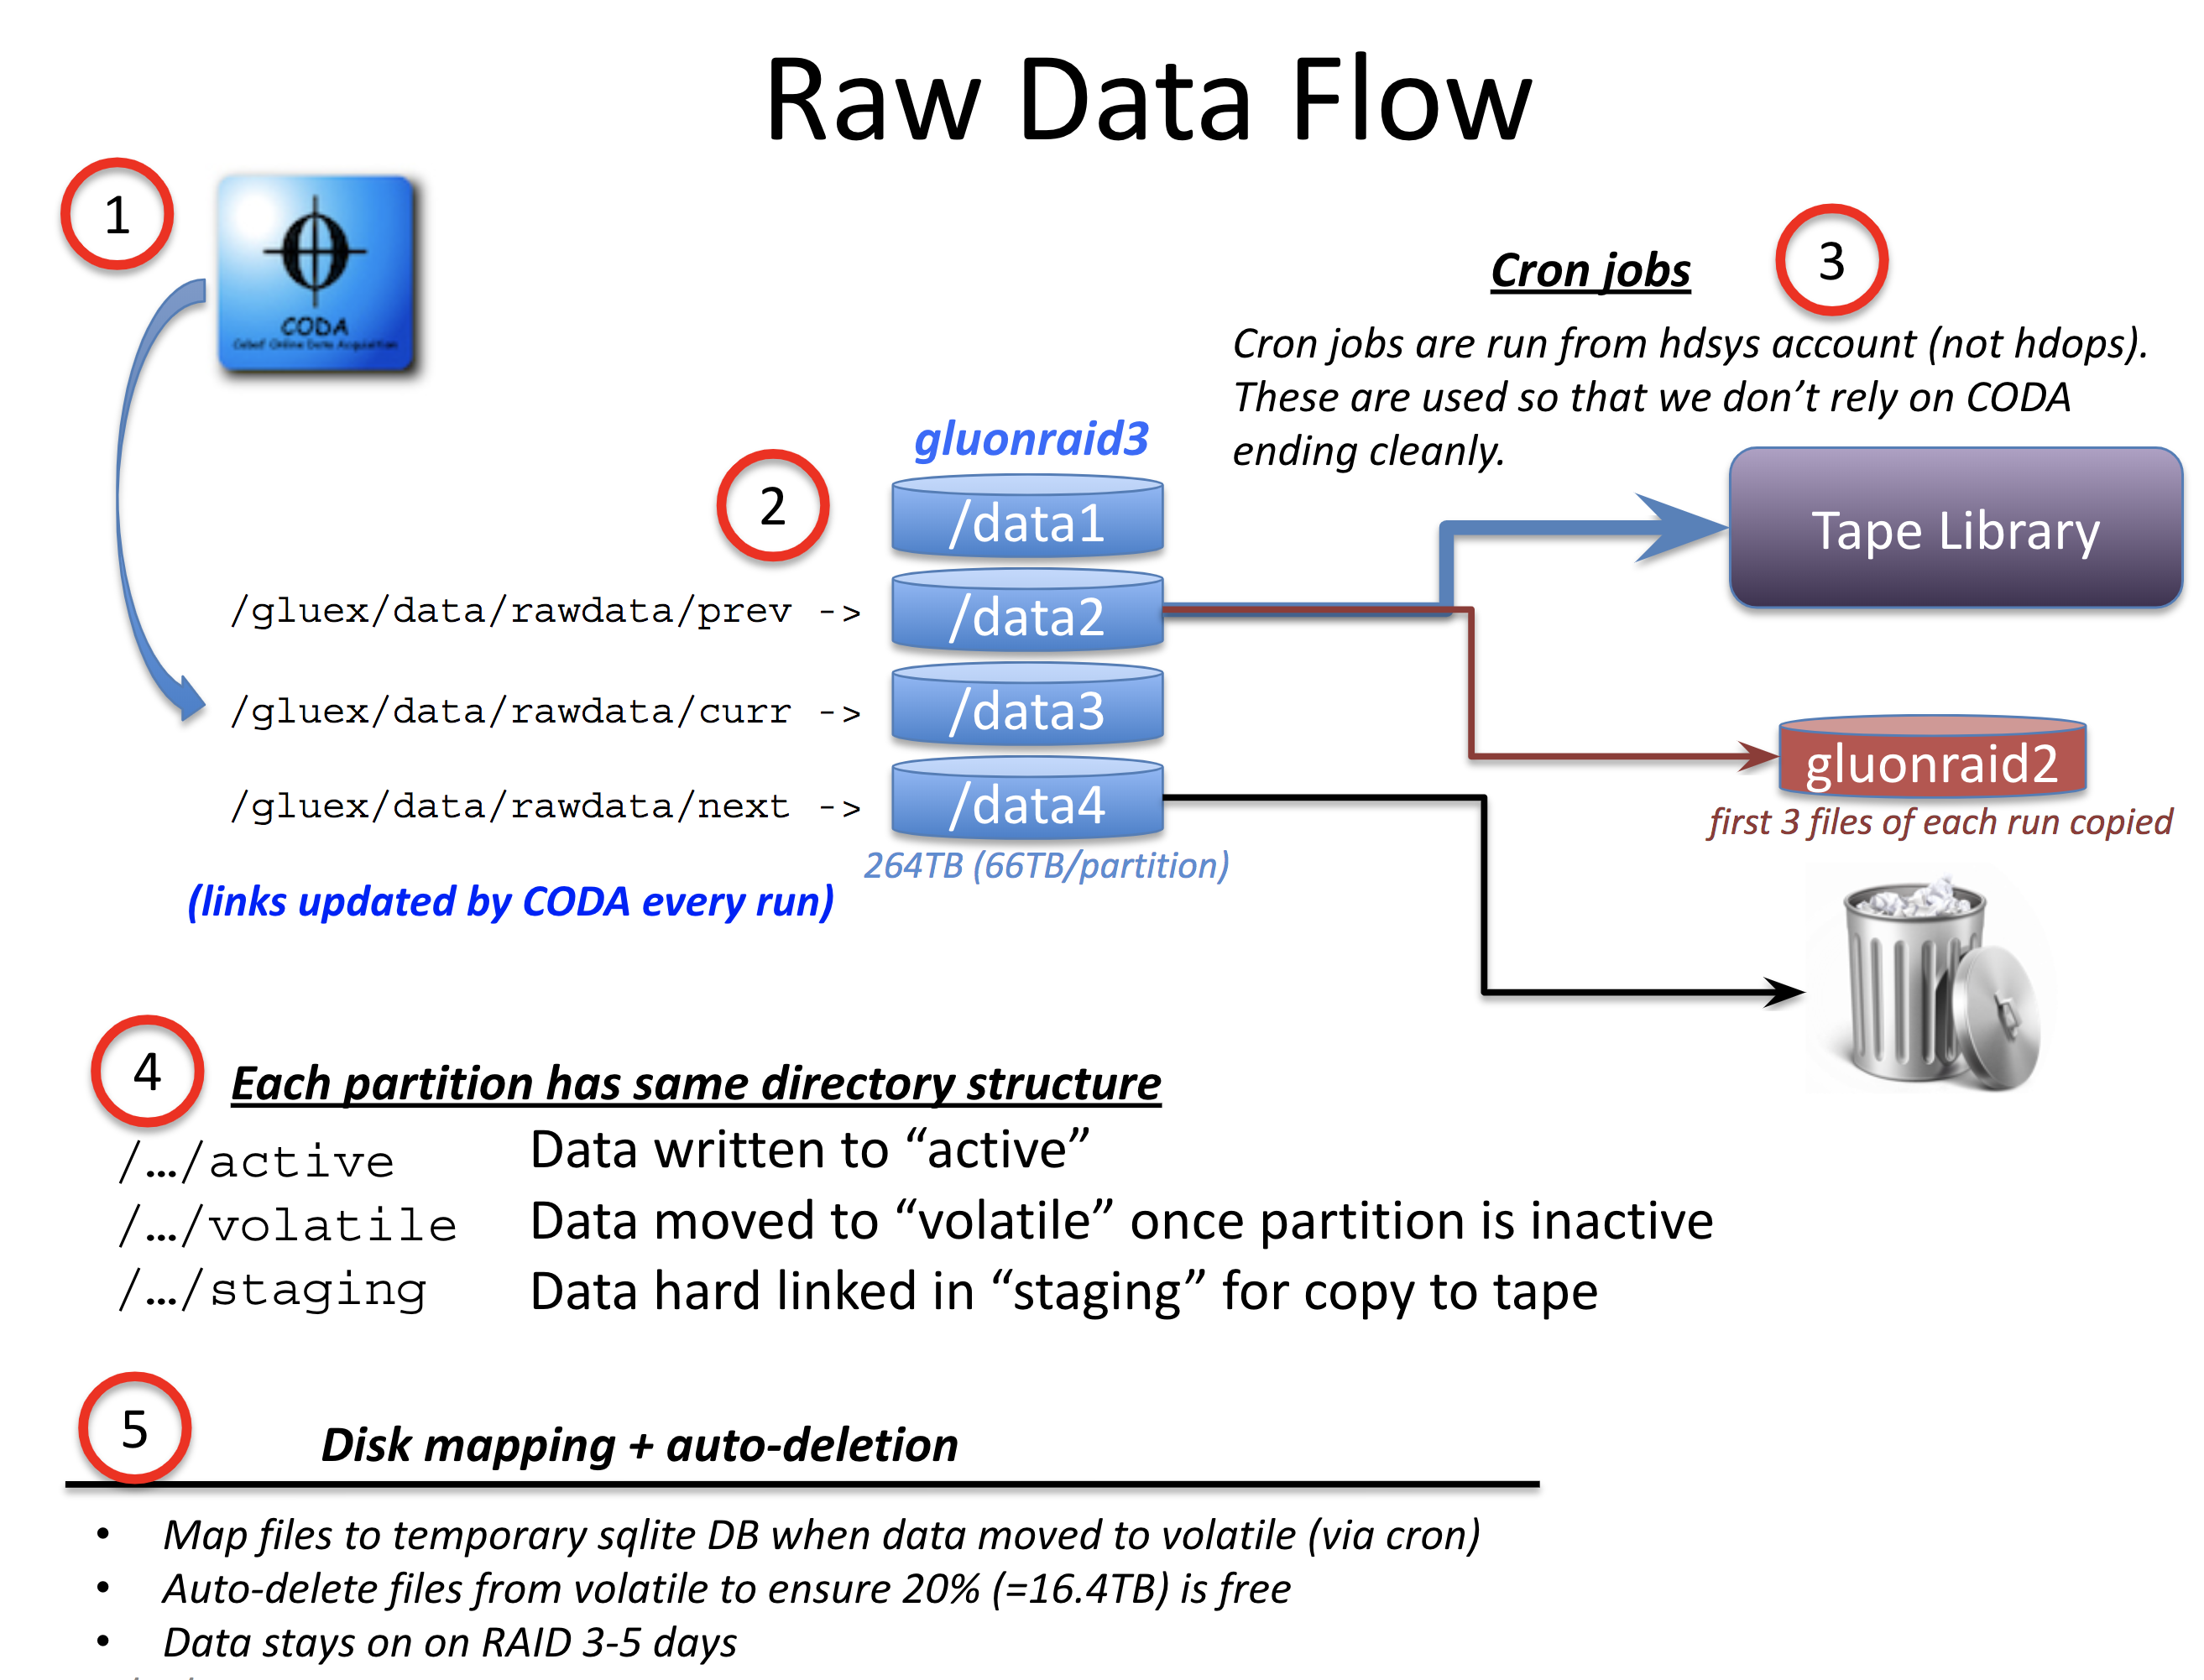
\includegraphics[width=0.99\textwidth]{figures/online_dataflow.png}
\caption{\label{fig:online_dataflow}Diagram of the data transport system used to move the data through the temporary RAID storage system to tape. The numbers with red circles given an indication of the sequence of the flow. }   
\end{center}  
\end{figure}
